\documentclass[Main.tex]{subfiles} 
\begin{document}

\subsubsection{Use Case 1.1: M�l og vej klods realisering}

M�l og vej klods Use Casen er realiseret p� s�dan en m�de, at systemet kalder ned i Data access layer som muligg�r kommunikation til robot dll'en. Her benytter den funktionen GetJaw(), hvorp� den f�r robotarmens klo aktuelle millimeter afstand. Denne funktion udf�res tre gange for at f� samtlige sider p� klodsen. 
Klodsen placeres ydermere p� v�gten, hvor systemet henter klodsens v�gt via Data access layer. Denne gang er det GetWeight() funktionen der kaldes. Her opn�s den nuv�rende v�gt. GetWeight() fungere ved at sende et kald ned til microcontrolleren der f�r denne til at konvenerer den p�g�ldende sp�nding fra strain-gauge-v�gten til en ADC-v�rdi, der returneres op til systemet. ADC-v�rdien omregnes via line�r regression til en v�gt m�lt i gram.
\\
Interaktionsdiagram over "M�l og vej klods":
\begin{figure}[H]
	\centering
	
	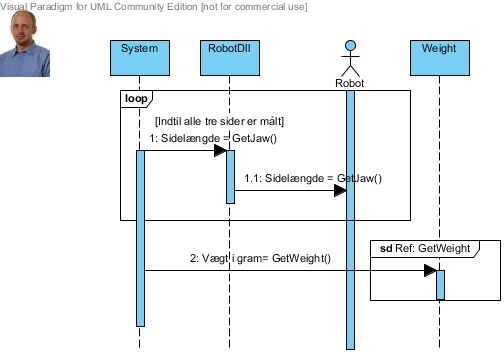
\includegraphics[scale=0.75, trim = 30mm 0mm 0mm 10mm, clip]{./Diagrammer/SSD/5_3_2_Use_Case_1_1_Maal_og_vej_klods_realisering_1.jpg}
	\caption{Simpelt sekvensdiagram af M�l og vej klods}
	\label{fig:5_3_2_Use_Case_1_1_Maal_og_vej_klods_realisering_1}
\end{figure}

Specificeret interaktionsdiagram af v�gten:
\begin{figure}[H]
	\centering
	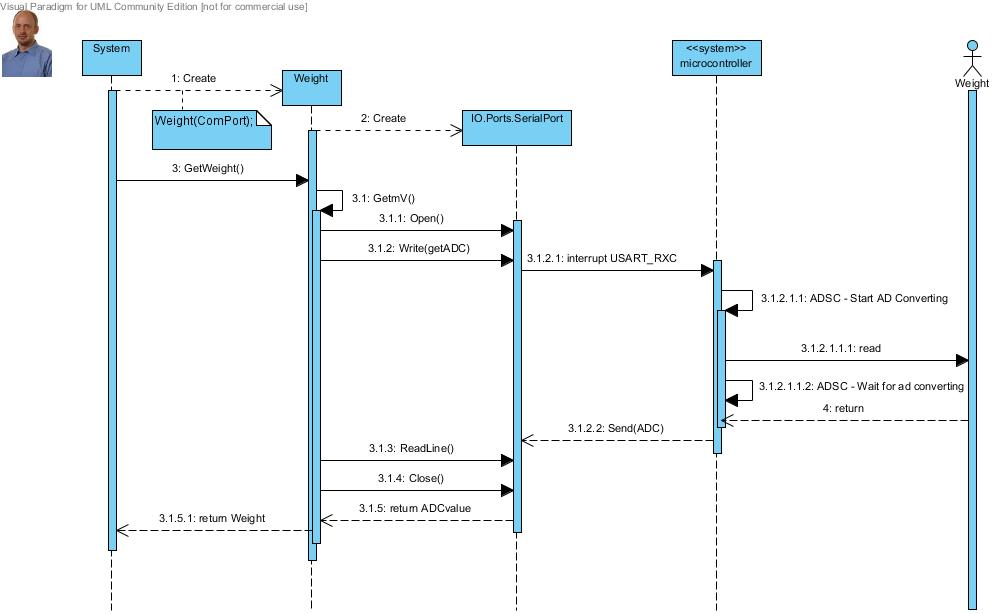
\includegraphics[scale=0.50, trim = 25mm 0mm 0mm 10mm, clip]{./Diagrammer/SSD/5_3_2_Use_Case_1_1_Maal_og_vej_klods_realisering_2_Weight.jpg}
	\caption{Detaljeret sekvensdiagram af v�gten}
	\label{fig:5_3_2_Use_Case_1_1_Maal_og_vej_klods_realisering_2_Weight}
\end{figure}
\end{document}